% -----------------------------------------------------------------------------
%   Arquivo: ./02-elementos-textuais/trabalhosRelacionados.tex
% -----------------------------------------------------------------------------

\chapter{Aprendizado de máquina}
\label{chap:MachineLearning}

\section{Formulação e caracterização do aprendizado de máquina}

Nos primórdios da inteligência artificial, pesquisadores foram capazes de resolver problemas que são intelectualmente difíceis para os seres humanos, mas relativamente simples para os computadores. Exemplo disso são os problemas que podem ser descritos por uma sequência de regras ou que podem ser solucionados por operações matemáticas \cite{Goodfellow-et-al-2016}.

A dificuldade surgiu para fazer com que os computadores fossem capazes de resolver tarefas fáceis para os humanos, mas difíceis de serem descritas de forma algorítmica, como reconhecer escrita, identificar rostos em imagens ou ainda definir regras de decisão de forma autônoma \cite{Goodfellow-et-al-2016}.

Eis que surgiu o campo de Aprendizado Máquina, uma alternativa que permitia computadores aprender por exemplo e não por regras. Ao reunir o conhecimento da experiência, esta abordagem evita a necessidade de operadores humanos especificar formalmente todo o conhecimento que o computador precisa. Isso ocorre através da combinação do aprendizado de conceitos simples, em formato pré-definido, combinados de forma hierárquica para formar um aprendizado de conceitos complicados \cite{Goodfellow-et-al-2016}.

Segundo \citeonline{Cherkassky2007}, o processo de aprendizado é definido como a estimação de uma relação ou estrutura, previamente desconhecida, entre entrada e saída. Segundo o autor, o processo de aprendizado normalmente envolve três componentes \ref{fig:MLFormulation} : o \textit{Gerador} de amostras, um \textit{Sistema} que gera as saídas reais e o \textit{Aprendizado de Máquina} que estima a relação desconhecida entre entrada e saída. 

\begin{figure}[!htb]
	\centering
	\caption{Formulação do Aprendizado} 
	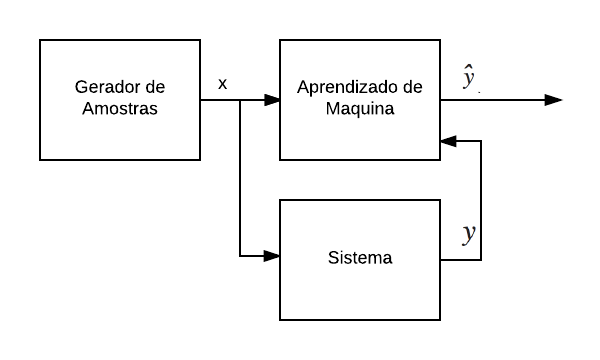
\includegraphics[width=0.8\textwidth]{./04-figuras/MLForm.png}
	\label{fig:MLFormulation}
\end{figure}

\citeonline{Cherkassky2007} explica que o \textit{Gerador} produz aleatoriamente, com distribuição de probabilidade $p(x)$, vetores $x \in {\mathbb {R}} ^{n}$, que são as características. O \textit{Sistema} é capaz de produzir, com probabilidade $p(y | x)$, saídas $y = g(x) + \epsilon$ em que $\epsilon$ é um ruido branco de $\mu = 0$. De forma geral, o \textit{Aprendizado de Máquina} é capaz de implementar uma função $\hat{y} = f(x, \omega)$, $\omega \in \Omega$, em que $\Omega$ é conjunto de parâmetros da função $f$.

O aprendizado de máquinas clássico diz respeito à aprender pelo exemplo, que é definido como um conjunto de dados, previamente obtidos pelo \textit{Gerador} e \textit{Sistema}, composto por variáveis quantitativas e qualitativas que são características do problema. Na situação onde existe uma variável resposta, o aprendizado é chamado de supervisionado, na situação onde essa variável não existe, o problema é definido como aprendizado não supervisionado. A figura \ref{fig:MLProblems} ilustra essa taxonomia, bem como algumas de suas subdivisões.


\begin{figure}[!htb]
	\centering
	\caption{Principais Problemas em Aprendizado de Máquina} 
	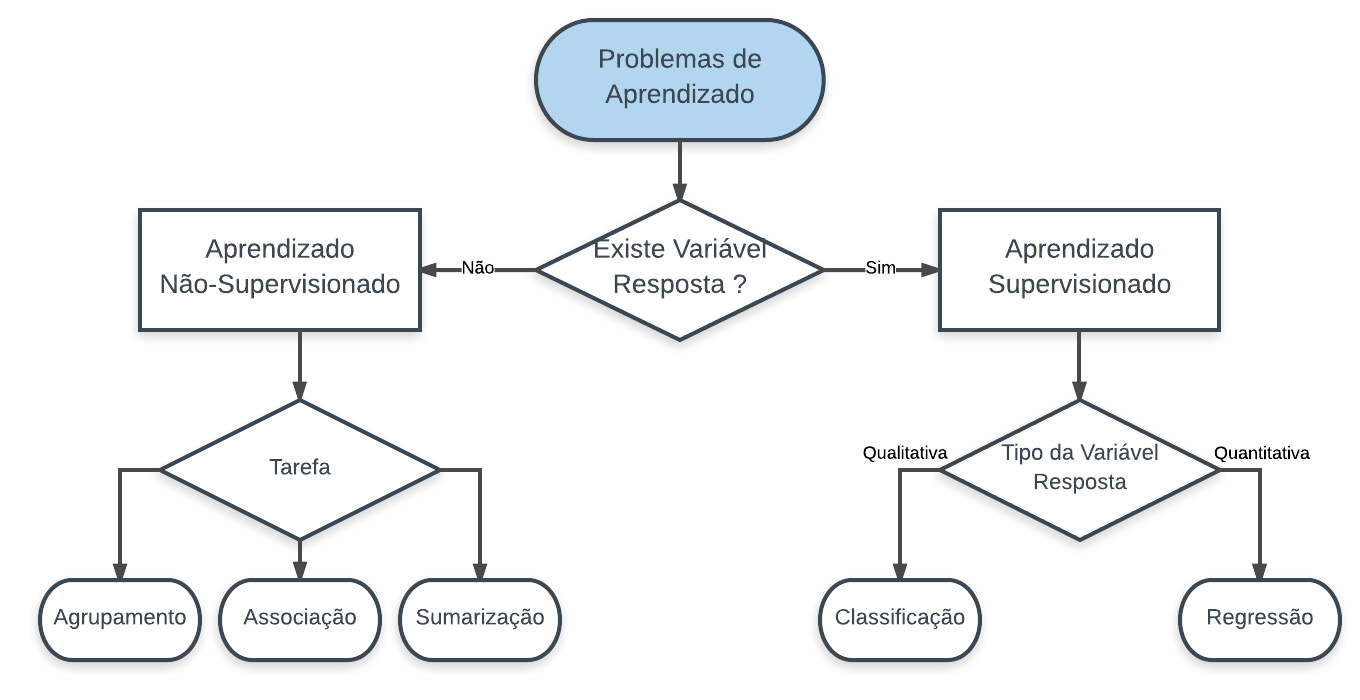
\includegraphics[width=0.8\textwidth]{./04-figuras/MLProblems.png}
	\label{fig:MLProblems}
\end{figure}
\section{Aprendizado supervisionado}

No aprendizado supervisionado, o objetivo é prever o valor de uma variável resultado com base em variáveis características. Na situação que a variável resposta é quantitativa, o problema é considerado como uma tarefa de regressão. Quando essa variável resposta é qualitativa, a tarefa é chamada de classificação.

De acordo com \citeonline{Cherkassky2007}, existem duas interpretações para o problema de aprendizado : identificação e imitação. A interpretação escolhida para fundamentar esse trabalho é a de imitação, descrita por \citeonline{Vapnik1971}.

O objetivo do aprendizado é encontrar uma função $f(x, \omega)$ que aproxima, da melhor forma possível, a saída $y$ do \textit{Sistema}. Para formular esse problema matematicamente, \citeonline{Cherkassky2007}, assumem pares de características e respostas, $(x_i, y_i)$ em que $i = (1, 2, ..., n)$ e $ n \in \mathbb {N}$, e uma função de custo $L(y, f(x, \omega))$que mede a discrepância entra saída do \textit{Sistema} $y$ e do \textit{Aprendizado de Máquina} $\hat{y}$. Então, formulam que a tarefa do aprendizado é descrita pela equação \ref{eq:LearningEq} . 

\begin{equation}
{	
	{\displaystyle {\underset {f}{\operatorname {arg\,min} }}\, L(y, f(x, \omega))}
}
\label{eq:LearningEq}
\end{equation}

A principal diferença entre problemas de classificação e regressão é a função de custo. Como a variável de saída de cada um desses problemas tem um formato diferente, a função de custo deve ser adaptada especificadamente para ele. Contudo, a formulação do aprendizado feito na equação \ref{eq:LearningEq} permanece inalterada, pois o objetivo é sempre minimizar a discrepância entre \textit{Sistema} e \textit{Aprendizado de Máquina} \cite{Cherkassky2007}.

\subsection{Problemas de classificação}
A situação mais simples de classificação é aquele em que a saída $y$ assume apenas dois valores, $y = 0$ ou $y = 1$, em que é chamada de problema de classificação binária. Nessa situação, segundo \citeonline{HastieFerro}, a função de custo específica é do formato \ref{eq:ClassProb}.

\begin{equation}
{	
	 L(y, f(x, \omega)) = \begin{dcases*}
	0,  & se $y = f(x, \omega)$ \\
	l,  & se $y \ne f(x, \omega)$ 
	\end{dcases*} \\ 
	l \in \mathbb {R^+}
}
\label{eq:ClassProb}
\end{equation}

O senário em que $y$ assume $q$ valores, em que $q > 2 \land q \in \mathbb {N}$, chamada de classificação \textit{multilabel}, pode ser simplificado em $q$ problemas de classificação binária em que o problema $j$ tem forma $y = j \rightarrow y_j = 1$ e $y_j \neq  \rightarrow y_j = 0 $, para $ 0 \leq j \leq q \land j \in \mathbb {N}$.


\subsection{Problemas de regressão}
O problema de regressão é caracterizado, segundo \citeonline{HastieFerro}, por $y \in \mathbb {R}$, dessa forma a função de custo normalmente é formulada como mostra a equação \ref{eq:RegProb}, onde $d$ é uma métrica genérica de distância entre dois números reais.

\begin{equation}
L(y, f(x, \omega)) = d(y, f(x, \omega))
\label{eq:RegProb}
\end{equation}

Nessa sistuação a variável de saída $y$ assume qualquer valor real, e a função $f$ mapeia a relação, linear ou não-linear, entre a entrada $x$ e essa saída.


\section{Métodos de Classificação} 
Nesse capítulo serão abordados os métodos de classificação implementados no pacote MLAT \cite{PauloCirinoMLAT}. 

\subsection{\textit{k Nearest Neighbours}}
O método \textit{k Nearest Neighbours} (\textbf{kNN}) é o algoritmo não paramétrico de classificação mais simples e conhecido \cite{James20131} . Seu funcionamento se dá de forma que a predição de uma amostra desconhecida é a moda das $k$ amostras mais próximas. De forma genérica sua implementação pode ser feita utilizando o pseudocódigo abaixo adaptado do trabalho de \citeonline{articleTay} :

\begin{algorithm}
	\caption{Algoritmo k-\textit{Nearest Neighbours}}
	\KwIn{$x$ amostra desconhecida,  $k$ é o parâmetro do número de vizinhos, $\{\mathbb{X}, \mathbb{Y}\}$ é o conjunto de pares amostras e respostas conhecidas }
	\KwOut{a predição da amostra desconhecida $y$ }
	
	\For {\textbf{each} $x_i \in \mathbb{X}$} {
		Computa a distância da amostra conhecida $i$ para a desconhecida $\mathbb{D_i} = d(x, x_i)$ \\
	}
	Seleciona o conjunto $\mathbb{L}$ referente as $k$ respostas com menor distância $\mathbb{D}$, onde $\mathbb{L} \in Y$ \\ 
	Computa a resposta $y = moda(\mathbb{L})$
\end{algorithm}
 

É importante ressaltar algumas características do kNN, como sua simplicidade de implementação e a não existência de uma etapa de treinamento. Além disso, o método é capaz de produzir superfícies de decisão não lineares e é robusto, dado uma escolha adequada do parâmetro $k$, a conjuntos ruidosos.

Entretanto esse algoritmo se baseia na memória das amostras conhecidas, fazendo com que ele não seja capaz de generalizar sua superfície de decisão para novas amostras fora do espaço conhecido. Outra consequência de ser um sistema baseado em memória é sua complexidade $O(n)$, para espaço e tempo, no momento de predição de cada uma das amostras de teste. 


\subsection{\textit{Support Vector Machines}}
As \textit{Support Vector Machines}, em português Máquinas de Vetor de Suporte, foram inicialmente propostas em \citeonline{boser1992training}. Esse método foi produzido como uma alternativa que, diferente de outros algoritmos tradicionais, não minimiza o erro do classificador, mas, sim maximiza a margem de separação entre duas classes \cite{James20131}. O intuito disso é produzir um classificador que seja capaz de encontrar uma superfície de decisão mais genérica, e consequentemente, que tenha melhor desempenho em amostras desconhecidas \cite{Cortes1995}.

A formulação inicial dessa metodologia sofreu adaptações e melhorias ao longo do tempo, em \citeonline{boser1992training} o classificador possuía margem rígida e assumia que existia uma superfície que separasse perfeitamente as classes, chamado hoje de \textit{Hard Margin SVM}.

Dado um conjunto de pares $(x_i, y_i)$ é possível formular esse classificador conforme a equação \ref{eq:SVMSeparavel} \cite{James20131}. Nessa formulação as respostas são $y_i \in \{1, -1\}$, $(\beta_0 + \sum_{j=1}^{p}{{\beta_i x_{ij}}})$ é o hiperplano de separação e $M$ é a variável de otimização que diz respeito ao tamanho da margem. 

\begin{equation}
\begin{split}
\underset {\beta_0, \beta_1, ..., \beta_p, M}  {\text{Maximizar : }} &{M} \\
\text{Sujeito a : } \\
&\sum_{j=1}^{p}{{\beta_j}^2} = 1, \\
&y_i(\beta_0 + \sum_{j=1}^{p}{{\beta_i x_{ij}}}) \geq M, \forall i = 1, ..., n
\end{split}
\label{eq:SVMSeparavel}
\end{equation}

Em \citeonline{Cortes1995} é demostrada uma alteração na formulação original, fazendo ser possível encontrar uma solução mesmo em problemas que as amostras não sejam completamente separáveis. Isso é feito por meio da introdução de um parâmetro $\epsilon_i$, que diz respeito a penalidade de amostras classificadas erroneamente. Essa alteração na formulação, conhecida como \textit{Soft Margin} SVM, é demonstrada pela equação \ref{eq:SVMInseparavel} \cite{James20131}.

\begin{equation}
\begin{split}
\underset {\beta_0, ..., \beta_p, \epsilon_1, ..., \epsilon_n, M}  {\text{Maximizar : }} &{M} \\
\text{Sujeito a : } \\
&\sum_{j=1}^{p}{{\beta_j}^2} = 1, \\
&y_i(\beta_0 + \sum_{j=1}^{p}{{\beta_i x_{ij}}}) \geq M(1 - \epsilon_i), \forall i = 1, ..., n, \\
&\epsilon_i \geq 0,  \sum_{i=1}^{n}{\epsilon_i} \geq C
\end{split}
\label{eq:SVMInseparavel}
\end{equation}

As equações \ref{eq:SVMSeparavel} e \ref{eq:SVMInseparavel} definem modelos de aprendizado com uma superfície de decisão linear. Para solucionar essa questão foi introduzido, em \citeonline{boser1992training} , o conceito conhecido como \textit{Kernel Trick}.

A implementação do \textit{Kernel Trick} é feita substituindo o produto interno, $f(x) = \beta_0 + \sum_{j=1}^{p}{{\beta_i x_{ij}}}$ por uma função genérica $K(x_i)$ não linear \cite{James20131}. Essa função pode introduzir termos de ordem superior ou até mesmo aplicar funções não lineares, tudo com o objetivo de facilitar a separabilidade das amostras. 
	
\subsection{\textit{Multilayer Perceptron}}
\label{sssec:MLPClassificationSubSection}
Uma rede neural artificial é formada por um conjunto de nodos, chamados de neurônios, com capacidade de processamento local e independe, agrupados em uma topologia definida \cite{Braga2007}.  O modelo \textit{Multilayer Perceptron} (MLP) é um tipo de rede neural artificial \textit{feedfoward}, que utiliza em sua camada intermediária neurônios perceptron \cite{AbadiABBCCCDDDG16}. 

\begin{equation}
y = \phi(\sum_{i = 1}^{m}{x_i  w_i} + b)
\label{eq:perceptron}
\end{equation}

O neurônio perceptron, definido pela equação \ref{eq:perceptron}, é o resultado da combinação linear dos termos das entradas $x_i$ ponderados por pesos$w_i$ e um bias $b$, após a introdução de uma não linearidade pela função de ativação $\phi$. A função de ativação $\phi$ pode assumir formatos diferentes, todavia, tradicionalmente ela é logística, tangente hiperbólica ou RELU conforme equações \ref{eq:act1}, \ref{eq:act2} e \ref{eq:act3} respectivamente \cite{Goodfellow-et-al-2016}.

\begin{equation}
\phi(z) = \frac{1}{1 + e^{-z}}
\label{eq:act1}
\end{equation}

\begin{equation}
\phi(z) = \frac{e^z - e^{-z}}{e^z + e^{-z}}
\label{eq:act2}
\end{equation}

\begin{equation}
\phi(z) = max(z, 0)
\label{eq:act3}
\end{equation}
%

A topologia da MLP, ilustrada na imagem \ref{fig:MLPDraw}, é compostas por 3 tipos de camadas : entrada, intermediária ou escondida, e, saída  \cite{Braga2007}. A rede possui uma camada de entrada com tamanho definido pelo número de variáveis do espaço dos dados de entrada. Ela pode possuir uma ou mais camadas intermediárias, formadas por neurônios perceptron, de tamanhos parametrizados por seu projetista. 

\begin{figure}[!htb]
	\centering
	\caption{Formulação do Aprendizado} 
	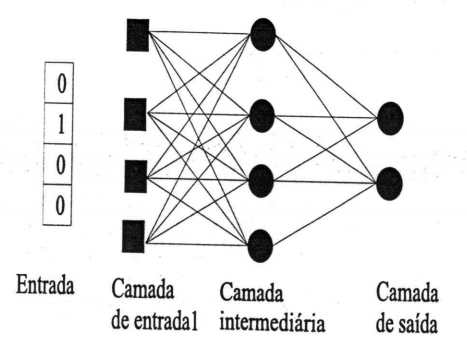
\includegraphics[width=0.8\textwidth]{./04-figuras/mlp.png} \\
	\cite{Braga2007}
	\label{fig:MLPDraw}
\end{figure}

A camada de saída em um problema de classificação, também pode assumir formatos diferentes. Para um problema binário, tradicionalmente é utilizado um neurônio do tipo logística, conforme equação \ref{eq:act1}.  No caso de problemas de classificação em que a saída pode assumir mais de 2 valores, a camada de saída deve possuir o mesmo  número de neurônios que valores de saída possíveis. Caso o projetista deseje ainda uma saída probabilística, é possível utilizar uma camada final do tipo \textit{softmax} conforme equação \ref{eq:softmax}, em que $k$ representa cada neurônio da camada de saída \cite{Goodfellow-et-al-2016}.  

\begin{equation}
\label{eq:softmax}
\sigma (\mathbf {z} )_{j}={\frac {e^{z_{j}}}{\sum _{k=1}^{K}e^{z_{k}}}}
\end{equation}

\section{Métodos de Regressão}
Nesse capítulo serão abordados os métodos de regressão implementados no pacote MLAT \cite{PauloCirinoMLAT}. 


\subsection{Regressão Linear}
O método de regressão linear é uma forma simples de performar aprendizado supervisionado, ainda assim, é um ótimo ponto de início para \textit{benchmarking} de modelos mais complicados de regressão. 

Em suma esse modelo encontra um vetor de pesos $W$ e um bias $b$ que melhor explica uma relação linear entre a entrada $x$ e a saída $y$, conforme a equação \ref{eq:LinearRegressionModel}.

\begin{equation}
\hat{y}= {x \cdot W^T} + b
\label{eq:LinearRegressionModel}
\end{equation}

Para estimar o vetor de pesos e o termo de bias é formulado um problema de otimização que minimiza a soma dos quadrados do erro residual, conforme equação  \ref{eq:LinearOpt}, utilizando o método de mínimos quadrados \cite{James20131}.

\begin{equation}
\underset {W, b}{\operatorname {arg\,min} }\ \sum_{i=1}^{n} ({y_i -  (x_i \cdot W^T+ b) })^2
\label{eq:LinearOpt}
\end{equation}

\subsection{\textit{Ridge Regression}}
\textit{Ridge Regression} é um modelo de aprendizado muito parecido com a regressão linear, a única diferença é que existe um termo adicional na função objetivo para minimizar a norma dos pesos $w_j \in W$, conforme mostra a formulação \ref{eq:LinearOptRidge} \cite{James20131} .

\begin{equation}
\underset {W, b}{\operatorname {arg\,min} }\ \sum_{i=1}^{n} ({y_i -  x_i \cdot W^T- b })^2 +  \lambda \sum_{j=1}^{m} {w_j}^2
\label{eq:LinearOptRidge}
\end{equation}

O termo $\lambda$ da equação, chamado de termo de penalização, não é otimizado pelo método, mas sim, é um parâmetro escolhido pelo projetista. Esse termo é sempre $\lambda \geq 0$, e quanto maior $\lambda$, mais os pesos referentes as variáveis não importantes são próximos de $0$ \cite{Wieringen2015}. Um caso especial desse termo é $\lambda = 0$, em que a \textit{ridge regression} se torna exatamente igual a uma regressão linear.

Dessa forma, o método de \textit{ridge regression}, têm uma tendência de generalizar melhor o aprendizado em situações em que existem muitas variáveis de entradas que não adicionam informações ao modelo \cite{Wieringen2015}.

\subsection{\textit{Multilayer Perceptron}}
Na seção \ref{sssec:MLPClassificationSubSection} foi definida a topologia da rede neural artificial MLP para o problema de classificação, entretanto, esse método também pode ser utilizado para problemas de regressão.

Nessa situação as camadas de entrada e intermediária permanecem exatamente iguais, a única mudança necessária é na camada de saída. Para regressão a camada de saída é um único neurônio linear conforme mostrado pela equação \ref{eq:neuronLinear} \cite{Goodfellow-et-al-2016}.  

\begin{equation}
\phi(z) = z
\label{eq:neuronLinear}
\end{equation}

